% !TEX root = ../double_trouble_main.tex

We next check the quality of our predictions experimentally. First we check that our method performs well on well-specified synthetic data, as well as some particular forms of misspecification. Then we see that our method provides high-quality predictions on a real human cancer genetics dataset and a real human genomic dataset. Throughout, we illustrate the advantages of modeling two populations together rather than treating the two populations separately or all from a single population.

\paragraph{Experimental setup.} In all of our experiments, we will have access to a collection of genetic samples for each of two populations (e.g., two types of cancer). Our validation procedure is reminiscent of cross-validation and analogous to the single population validation procedures of \citet{Masoero2022,  zou2016quantifying}. Within each population, we uniformly at random choose a partition of the data into 20 equally-sized blocks. \minorrevision{Since the dataset size may not be a multiple of 20, block sizes in practice may vary by 1. We will elide  small details of this form in the remainder of this section for clarity of exposition. Also, the population genetics data is substantially larger than our other datasets, so --- to avoid a very large pilot size --- we use 30-fold cross-validation in that case (\cref{sec:real_data}).} 

In each of 20 folds, we reserve one block (unique to this fold) to be the pilot data for its corresponding population, so the final pilot sample has size $\vecsamplesize = (\samplesize{1}, \samplesize{2})$. The remaining data will serve as potential follow-up data. Each method has access only to the pilot data (across both populations), and we use the follow-up data (across both populations) to evaluate the accuracy of each method. None of the methods we consider in this paper use ordering information on the pilot data, but to generate all of our figures, we choose an ordering on the pilot data uniformly at random. Likewise, we choose an ordering on the follow-up data uniformly at random. In our figures, we present first the pilot data from population 1, then the pilot data from population 2, then the follow-up data from population 1, then the follow-up data from population 2. We can think of these figures as encapsulating a series of evaluations as follows. We train every method on the full pilot data in populations 1 and 2. Then we progressively test on follow-up sample sizes $\vecfuturesamplesize = (\futuresamplesize{1},\futuresamplesize{2})$ of the following forms: $(1,0), (2,0), \ldots, (19 \samplesize{1},0), (19 \samplesize{1},1), (19 \samplesize{1},2), \ldots, (19 \samplesize{1}, 19 \samplesize{2})$. In this way, we capture a wide range of ratios between follow-up sample sizes across the two populations: from all follow-up data in a single population to a ratio of follow-up sizes that matches the ratio in the pilot.
To summarize our results across all 20 folds, we will show an empirical mean across folds, both for each prediction method as well as for the ground truth. And we will show a shaded one-standard deviation interval for the prediction methods. The ground truth showed very small variation across folds so the interval appears almost invisible. %\tb{ultimately we will say something about ground truth here too once the results are in.} %\tb{Are the intervals for the ground truth very small? can we say something here?}

Recall that we are also interested in predicting the number of $\vecoccurrence$-tons in a follow-up sample of size $\vecfuturesamplesize$ (\cref{eq:news_freq}); that is, we are interested in predicting the number of new variants appearing exactly $\vecoccurrence$ times across the two populations. To evaluate our prediction in this case, we consider just the extreme where we use all possible data in the follow-up. For each value of $\vecoccurrence$ with $\occurrence{1}, \occurrence{2}$ each less than a threshold, we compute the \emph{relative residual}: namely, the signed difference between a method's prediction and the observed value in the reserved follow-up data, normalized by the observed value. We plot an empirical average of this quantity across the folds. We also report the actual observed values and absolute (un-normalized) residuals in Section S7.3 in the Supplementary Material \citep{supplement}, again averaged across the folds.

\paragraph{Comparisons.} To the best of our knowledge, there are no alternative methods for the prediction task we are interested in here. However, there are a number of methods that predict the number of variants in a follow-up given pilot data in a single population~\citep{Masoero2022, chakraborty2019using,gravel2014predicting}. So we consider two natural competitors in our experiments. First, we define the \emph{independent} two-population \revision{application} of a single-population method as follows. Given $\vecsamplesize$ pilot samples and $\vecfuturesamplesize$ follow-up samples, we train the single-population method first on the $\samplesize{1}$ pilot samples from population 1 and predict the number of variants expected in $\futuresamplesize{1}$ follow-up samples from population 1. We separately train the single-population method on the $\samplesize{2}$ samples from population 2 and predict the number of variants expected in $\futuresamplesize{2}$ follow-up samples from population 2. We report the sum of the predicted number of variants across both populations as the final prediction. 
In general, we expect the independent method to overcount the number of variants when there are follow-up samples from both populations. We do not include the independent method below when we compare performance in predicting $\vecoccurrence$-tons. In particular, whenever both elements of $\vecoccurrence$ are strictly positive, the independent method predicts there are zero $\vecoccurrence$-tons. We provide the \revision{prediction, its supporting theory, and how we perform hyperparameter selection} in Section S4.2 of the Supplementary Material of \citep{supplement}. In the real data we analyze at the sizes we consider, this zero prediction is unrealistic; see Figures S8 and S9 in the Supplementary Material \citep{supplement} for the ground-truth real-data $\vecoccurrence$-ton values. %(Also, see \cref{supp-fig:proposed_kton,supp-fig:i3BP_kton,supp-fig:d3BP_kton} for the ground-truth synthetic $\vecoccurrence$-ton values.)

%The independent method essentially assumes each variant is unique to a single population. From that perspective, when $\vecoccurrence = (\occurrence{1},0)$, we can take the population-1 prediction for the number of $\occurrence{1}$-tons and use it as the independent-method prediction for the number of $\vecoccurrence$-tons; an analogous prediction holds when $\occurrence{1} = 0$ and $\occurrence{2} > 0$. Whenever both elements of $\vecoccurrence$ are strictly positive, the independent method predicts there are zero $\vecoccurrence$-tons. In the real data we analyze at the sizes we consider, this zero prediction is unrealistic (see~\Cref{supp-fig:proposed_kton},~\ref{supp-fig:i3BP_kton},~\ref{supp-fig:d3BP_kton} for raw number of $\vecoccurrence$-tons in synthetic experiments and~\Cref{supp-fig:brca_luad_kton},~\ref{supp-fig:seu_bgr_kton} in real data experiments). 

Second, we define the \emph{dependent} two-population \revision{application} of a single-population method. In this case, we train the single-population method on all of the $\samplesize{1} +\samplesize{2}$ pilot samples, as though they are the pilot samples from a single population. To form a prediction on a follow-up sample of size $\vecfuturesamplesize$, we report the prediction on a single-population follow-up of size $\futuresamplesize{1} + \futuresamplesize{2}$. 
In general, we expect the dependent method to struggle when both (a) the two populations exhibit notably different variant growth rates and (b) the ratio of populations in the follow-up does not closely mirror the pilot \revision{because this mismatch exacerbates prediction errors. For example, if one population contains many rare variants while the other does not, changing the sampling proportions between pilot and follow-up will substantially impact variant discovery rates in ways the homogeneous model cannot account for.}
To predict the number of $\vecoccurrence$-tons, we predict the number of variants, conditional on the pilot, that we would expect to see $\occurrence{1}$ times out of $\futuresamplesize{1}$ follow-up samples and also $\occurrence{2}$ times out of $\futuresamplesize{2}$ distinct follow-up samples (all from the same assumed single population). For single-population methods that do not provide $\occurrence{}$-ton predictions (for scalar $\occurrence{}$), we will therefore not be able to provide $\vecoccurrence$-ton predictions in the dependent \revision{application}. 
However, we are able to provide $\vecoccurrence$-ton predictions for the special case of the single-population 3BP method due to \citet{Masoero2022}.
\internal{In particular, in Section S4.1 of the Supplementary Material \citep{supplement}, we describe how we modify \citet{Masoero2022} to predict vector-valued $\vecoccurrence$-tons; we provide theory analogous to \cref{prop:predict_kr_tons} and describe the method we employ to fit the hyperparameters}.
%\internal{see Section S4.1 of the Supplementary Material \citep{supplement} for a discussion on modifying \citet{Masoero2022} to predict vector values $\vecoccurrence$-tons, including supporting theory and the method employed to fit the hyperparameters}.

Since there are many single-population methods, in general we will select just one single-population method to use when reporting the independent and dependent results. In each case, we will try to use the single-population method that is best in a relevant sense, which we make precise in each case below.


\subsection{Synthetic experiments}
\label{sec:simulation}
% !TEX root = ../double_trouble_main.tex

We first confirm that our method is able to predict well on data simulated from our own model (\cref{eq:proposed_prior}), as a check on our methodology before moving to real data. To that end, we generate 500 data points in each of two populations; we describe the simulation procedure in more detail in~Section S6 of the Supplementary Material \citep{supplement}. So, in each of our 20 folds, the pilot data has size $\vecsamplesize = (25,25)$.

We simulate two different datasets from our model (\cref{eq:proposed_prior}); we choose the hyperparameters to reflect a range of growth rates, sample sizes, and correlations between the two populations in each case. We choose hyperparameters $\allhyper := (\mass, \rate{1},\rate{2}, \corr{1},\corr{2}, \conc{1},\conc{2}) = (100,0.4,0.6,0.5,0.5,1,1)$ for the first dataset and $\allhyper = (1,0.8,0.7,0.5,0.5,1,1)$ for the second dataset. We choose these values for qualitative matches with the observed variant growth in the GnomAD dataset (\cref{fig:pop_gen}) and cancer dataset (\cref{fig:cancer}), respectively. 

The results in \cref{fig:proposed} demonstrate that our method outperforms two potential baselines. Since here all of our data is simulated from our two-population BNP model, we use a single-population BNP model to form our baselines; namely, we compare to the independent and dependent two-population applications of the 3BP approach due to \citet{Masoero2022}. \internal{First, consider the simulation in the upper row of plots.} We see in the upper left plot in \cref{fig:proposed} that our method (solid red line) much more closely matches the behavior of the ground truth (dashed black line) than either the independent (dotted green line) or dependent (dash-dot blue line) applications. As expected, the independent application dramatically overcounts the number of variants in the second follow-up population. Also as expected, the dependent application performs well when the pilot and follow-up proportions are in agreement (at the largest sample size) but misestimates the number of variants elsewhere. By contrast, our method is able to capture the different behaviors of the two populations and account for any shared variants.

 In the lower left corner, the independent application of the 3BP performs the best; its mean line is closest to the ground truth, and its prediction exhibits the smallest variation (shaded range) across folds. Importantly, \internal{we can infer from the lower center plot that} there are extremely few shared variants in \internal{the simulation for the lower row}; see Section S7.3 of the Supplementary Material \citep{supplement} \internal{for raw observed and predicted counts.} That is, \internal{in the simulation for the lower row of plots,} the assumption of the independent application is very close to being correct. So, following Bayesian Occam's Razor \citep[ch.~28 p.~343]{mackaybook}, we expect better performance from the simpler model (the independent application) when its more stringent assumptions are true. That being said, our proposed model still performs well here; its mean line is also very close to the ground truth, by contrast to the dependent application. We conclude that our method is able to handle prediction of the number of new variants under a variety of two-population behaviors --- while the independent application is limited to the special cases where the two populations are known a priori to behave independently.

\begin{figure}[htp]
    \centering
    \includegraphics[width = 0.9\textwidth]{Figs/n3BP_20fold.png}
    \includegraphics[width = 0.9\textwidth]{Figs/n3BP_fast_20fold.png}
    \caption{Predictions when data is sampled from our model (\cref{eq:proposed_prior}). Each row corresponds to a simulated dataset (\cref{sec:simulation}). \emph{Left}: %The dashed black line shows the observed number of variants as a function of the sample number.
    The samples (horizontal axis) appear in the following order: pilot from population 1, pilot from population 2, follow-up from population 1, follow-up from population 2. A vertical dashed gray line separates the two populations in the pilot and follow-up, respectively. Vertical gray shading covers the pilot data. In the follow-up region, we plot mean (lines) and 1 standard deviation intervals (shaded regions) from ground truth (dashed black; also appears for the pilot) and three methods: our proposed method (solid red), the dependent version of the single-population 3BP (dash-dot blue), and the independent version of the 3BP (dotted green). \emph{Center and Right}: For each $\vecoccurrence$ with component values up to 10, we plot the relative residual for predictions from our method (right) and the dependent 3BP (center). \revision{Note: color scales are dataset-specific.} A square is gray when the observed value is strictly less than 2 in at least one fold or $\vecoccurrence = (0,0)$. 
    }
    \label{fig:proposed}
\end{figure}

From the center and right plots in \cref{fig:proposed}, we also see that our method provides better estimates of the numbers of various $\vecoccurrence$-tons. Recall that the independent application predicts zero for anything except private $\vecoccurrence$-tons, and we see that there are in fact non-trivial counts of shared $\vecoccurrence$-tons in the first data set. Given this limitation of the independent application, we focus on plotting results for our method and the dependent application. Darker colors indicate more erroneous predictions, so we conclude in both datasets that our method is providing more accurate predictions than the dependent 3BP application. Note that the observed numbers of $\vecoccurrence$-tons vary dramatically across $\vecoccurrence$ values. So generally we expect more noise in the upper right of our plots of $\vecoccurrence$-tons --- and should therefore take care not to treat every square in these plots equally. We can see the actual observation values for the two datasets in \internal{Fig. S5 (Section~S7.3)} of the Supplementary Material \citep{supplement}; in particular, for the first dataset, the observed number of $\vecoccurrence$-tons varies from an average (across folds) of 1161.2 at $(0,1)$ to 0 at various locations, e.g. (8,3), (10,4), and (7,7) (see the gray boxes in the upper left panel of \internal{Fig. S5 (Section~S7.3)} of the Supplementary Material \citep{supplement}).  We see similar behavior in the real data, as we describe below.

We check that our method is able to handle datasets generated from the (mis-specified) assumptions of the independent and dependent 3BP applications in Sections S7.1 and S7.5 of the Supplementary Material \citep{supplement}; \internal{in particular, in S7.5, we investigate a case where the data is generated from a dependent 3BP where the number of variants grows slowly, and using the independent 3BP for inference results in severe double counting of variants --- but our method continues to work well.}



\subsection{Real data}
\label{sec:real_data}
% !TEX root = ../double_trouble_main.tex

We next show that our method performs well on a real dataset in cancer genomics and semi-synthetic dataset in population genetics. We confirm that our method performs better than the independent and dependent applications of one-population methods.

\paragraph{Comparisons.} For the real datasets, we find that different one-population methods exhibit substantially different performance for different types of data. So, for each type of data (cancer, population genetics), we test a variety of different one-population methods. In Section S7.2 of the Supplementary Material \citep{supplement}, we compare them on the one-population task and choose the best-performing method to serve as the comparison (via independent and dependent applications) for our two-population method. \internal{In particular, we choose the one-population method with the lowest root mean squared error of the prediction curve for the number of variants; here, we take the mean across all values of the follow-up sample size (up to the largest value), and we note that this value depends on our choice of ordering of the data points.} For one-population methods, we consider the fourth-order jackknife \citep{burnham1978estimation, gravel2014predicting}, the Good-Toulmin estimator \citep{Orlitsky2016,chakraborty2019using}, linear programming \citep{zou2016quantifying}, the 3BP approach of \citet{Masoero2022}, and the scaled process of \citet{Camerlenghi2021}.


\paragraph{Two cancer genomic datasets.}
%
In cancer genomics, biologists are actively searching for (rare) shared genetic variants across cancer types that might lend insight into common causes of different cancers \citep{bojesen2013multiple, rashkin2020pan}. We next show that both our method and the independent application perform well at predicting the number of new variants, while the dependent application performs poorly. But unlike the independent application, our method is able to predict the (non-trivial) number of shared variants across populations -- and provides a better prediction than the dependent application.

In these experiments, we use the cancer genome atlas (TCGA) and MSK-IMPACT datasets \citep{cancer2008comprehensive, cancer2013cancer, cheng2015memorial}. 
We used the same processing as in \citet{chakraborty2019using} and \citet{Masoero2022}. 

To form our two populations, we focus on the two types of cancer with the largest numbers of samples; in each dataset, the resulting two types of cancer are lung cancer and breast cancer. In the MSK-IMPACT dataset, there are total of 749 lung cancer samples and 1532 breast cancer samples. In the TCGA dataset, there are total of 492 lung cancer samples and 811 breast cancer samples. So the pilot sizes are challenging in each case: 38, 57, 24, and 40, respectively.
%
For each population (lung cancer, breast cancer) in each dataset (TCGA, MSK-IMPACT), we find that the best-performing one-population method is the 3BP (Section S7.2 of the Supplementary Material \citep{supplement}). So we compare to the independent and dependent one-population applications of the 3BP in this analysis.



\begin{figure}[htp]
    \centering
    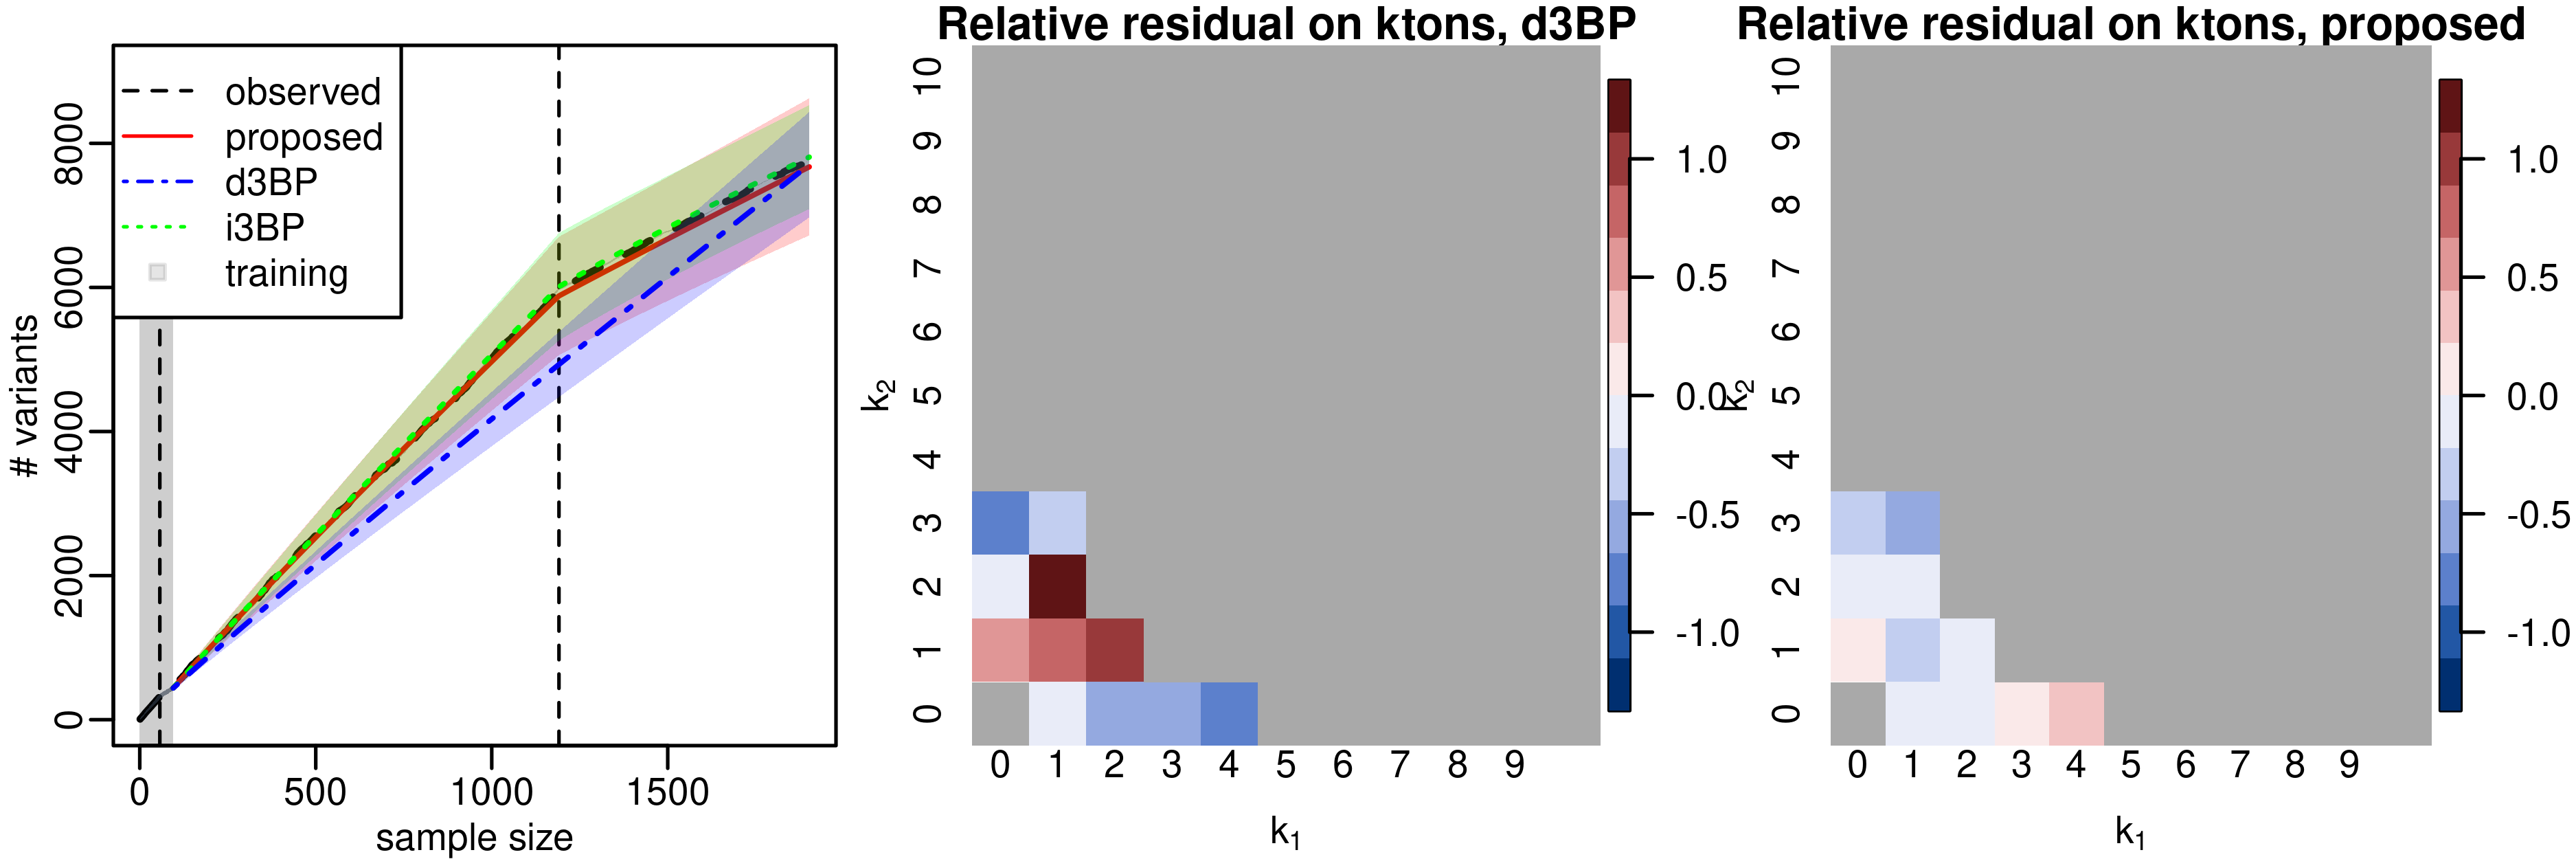
\includegraphics[width = 0.9\textwidth]{Figs/BIDC_LA2_20fold.png}
    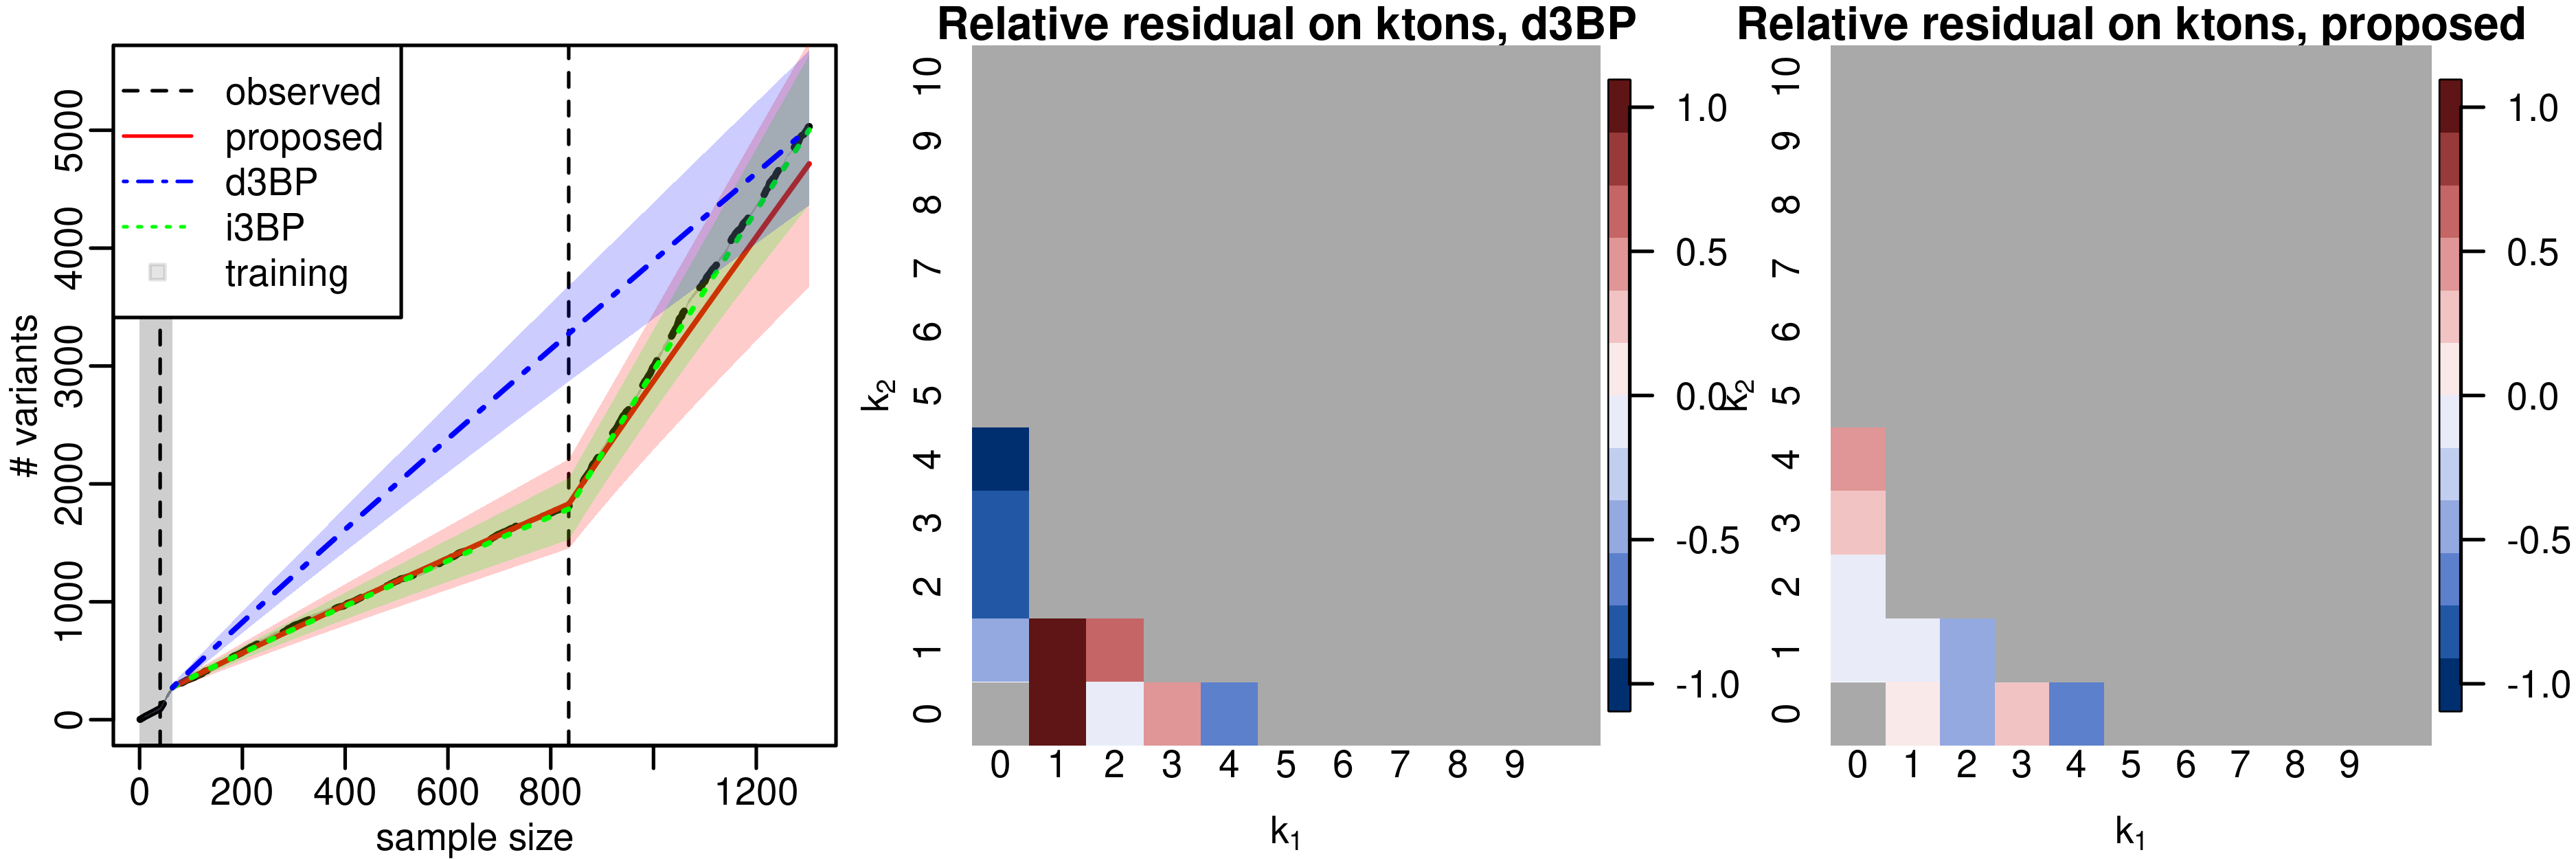
\includegraphics[width = 0.9\textwidth]{Figs/BRCA_LUAD_20fold.png}
    \caption{Predictions for the cancer genomics data. The rows correspond to datasets (upper: MSK-IMPACT, lower: TCGA). Population 1 is breast cancer, and population 2 is lung cancer. Other details of the plots are as in \cref{fig:proposed}.
    }
    \label{fig:cancer}
\end{figure}

The results in \cref{fig:cancer} demonstrate that our method outperforms the two one-population baselines. In particular, both our method and the independent application agree closely with the ground truth number of new variants across the various follow-up sizes (left panels). Indeed, we expect a low level of sharing between cancer types since most variants in cancer are \textit{de novo} variants -- not subject to the natural selection that might make variants more likely to be shared across populations. As expected the dependent application agrees with ground truth when the composition of the follow-up matches the pilot, but its predictions can be very far from the ground truth for other follow-up sizes. In the center and right plots, we see that there are still a number of shared variants with non-trivial counts in the ground truth; see also~Figure S8 of the Supplementary Material \citep{supplement} for direct plots of the ground truth. The independent application is unable to predict such counts. And while the dependent application can predict a non-zero number in these cases, we see from the center and right plots in \cref{fig:cancer} that our method's predictions are more accurate. Overall then, our method is the only one able to provide both useful predictions of the numbers of variants in a follow-up as well as useful predictions of the number of shared variants across populations in the follow-up.


\paragraph{A semi-synthetic population genetics dataset.}
%\label{sec:gnomad}

For population genetics, we use the GnomAD dataset \citep{karczewski2020mutational}. The dataset provides variant frequencies, but it does not provide exact variant data for each sample. So we take the semi-synthetic approach of \citet{Masoero2022}; namely, for each individual, we independently sample the presence of each variant according to the reported frequency of that variant in the data. In general, prediction is more challenging (a) when the pilot is small in absolute terms since less trend information is available 
and (b) when the follow-up is as large as possible since we have a priori more possibility for any observed trend to break down. To accomplish goal (b), we choose large populations: Korean (1909 samples), Bulgarian (1335), and Southern European (5752). We then choose 30 folds to ensure smaller pilots 
(64, 45, and 192, respectively), per goal (a).

For each population (Korean, Bulgarian, Southern European), we compare performance of the one-population \internal{methods listed at the start of} \cref{sec:real_data}; see Section S7.2 of the Supplementary Material \citep{supplement} \internal{for results}. For each population in this case, we find that the fourth-order jackknife (4JK) \internal{is the best performer}. So we use the 4JK for the independent and dependent one-population applications in this analysis.

The results in \cref{fig:pop_gen} demonstrate that our method outperforms the two one-population methods at predicting the number of new variants in a follow-up. When the follow-up composition matches the pilot (the most favorable case for the dependent application), our method is at least on par with the dependent one-population application at predicting the number of shared variants in a follow-up. 
We see in the upper left plot that the dependent application miscounts variants when the composition of the follow-up differs from the pilot. The independent application predicts the first population well but double counts shared variants when the second population appears in the follow-up. In the lower left, the two populations are more similar, so the dependent application performs reasonably; the independent application, though, double counts shared variants in the second population in the follow-up. In both examples, our method tracks closely with ground truth. 

In the upper center plot, we see that the dependent one-population application can be over an order of magnitude off in its predictions. In the upper right plot, we see that our method is much closer to ground truth across the $\vecoccurrence$ values here. Unlike in the cancer data case, the ground truth at all $\vecoccurrence$ values in this plot is substantially greater than zero; see Figure S8 of the Supplementary Material \citep{supplement} for more information about the ground-truth counts. In particular, the signed residual plot in Figure S8 of the Supplementary Material \citep{supplement} shows that the dependent application is providing an overestimate along the diagonal. Indeed, we expect that the Korean and Bulgarian populations have little overlap and thus few shared variants -- whereas the dependent application assumes they are the same population. Conversely, in the lower center and right plots, we see that our method is often farther from the ground truth than the dependent application. We note that the magnitude of the error is smaller than in the upper plots, but it is still quite high (larger than 100\%). It may be that the complex history between the related Southern European and Bulgarian populations cannot be captured by the simple models we consider here.  We reiterate that the independent application predicts zero for all $\vecoccurrence$ values that do not have a zero component and thus fails to predict all such values in these examples.






\begin{figure}[htp]
    \centering
    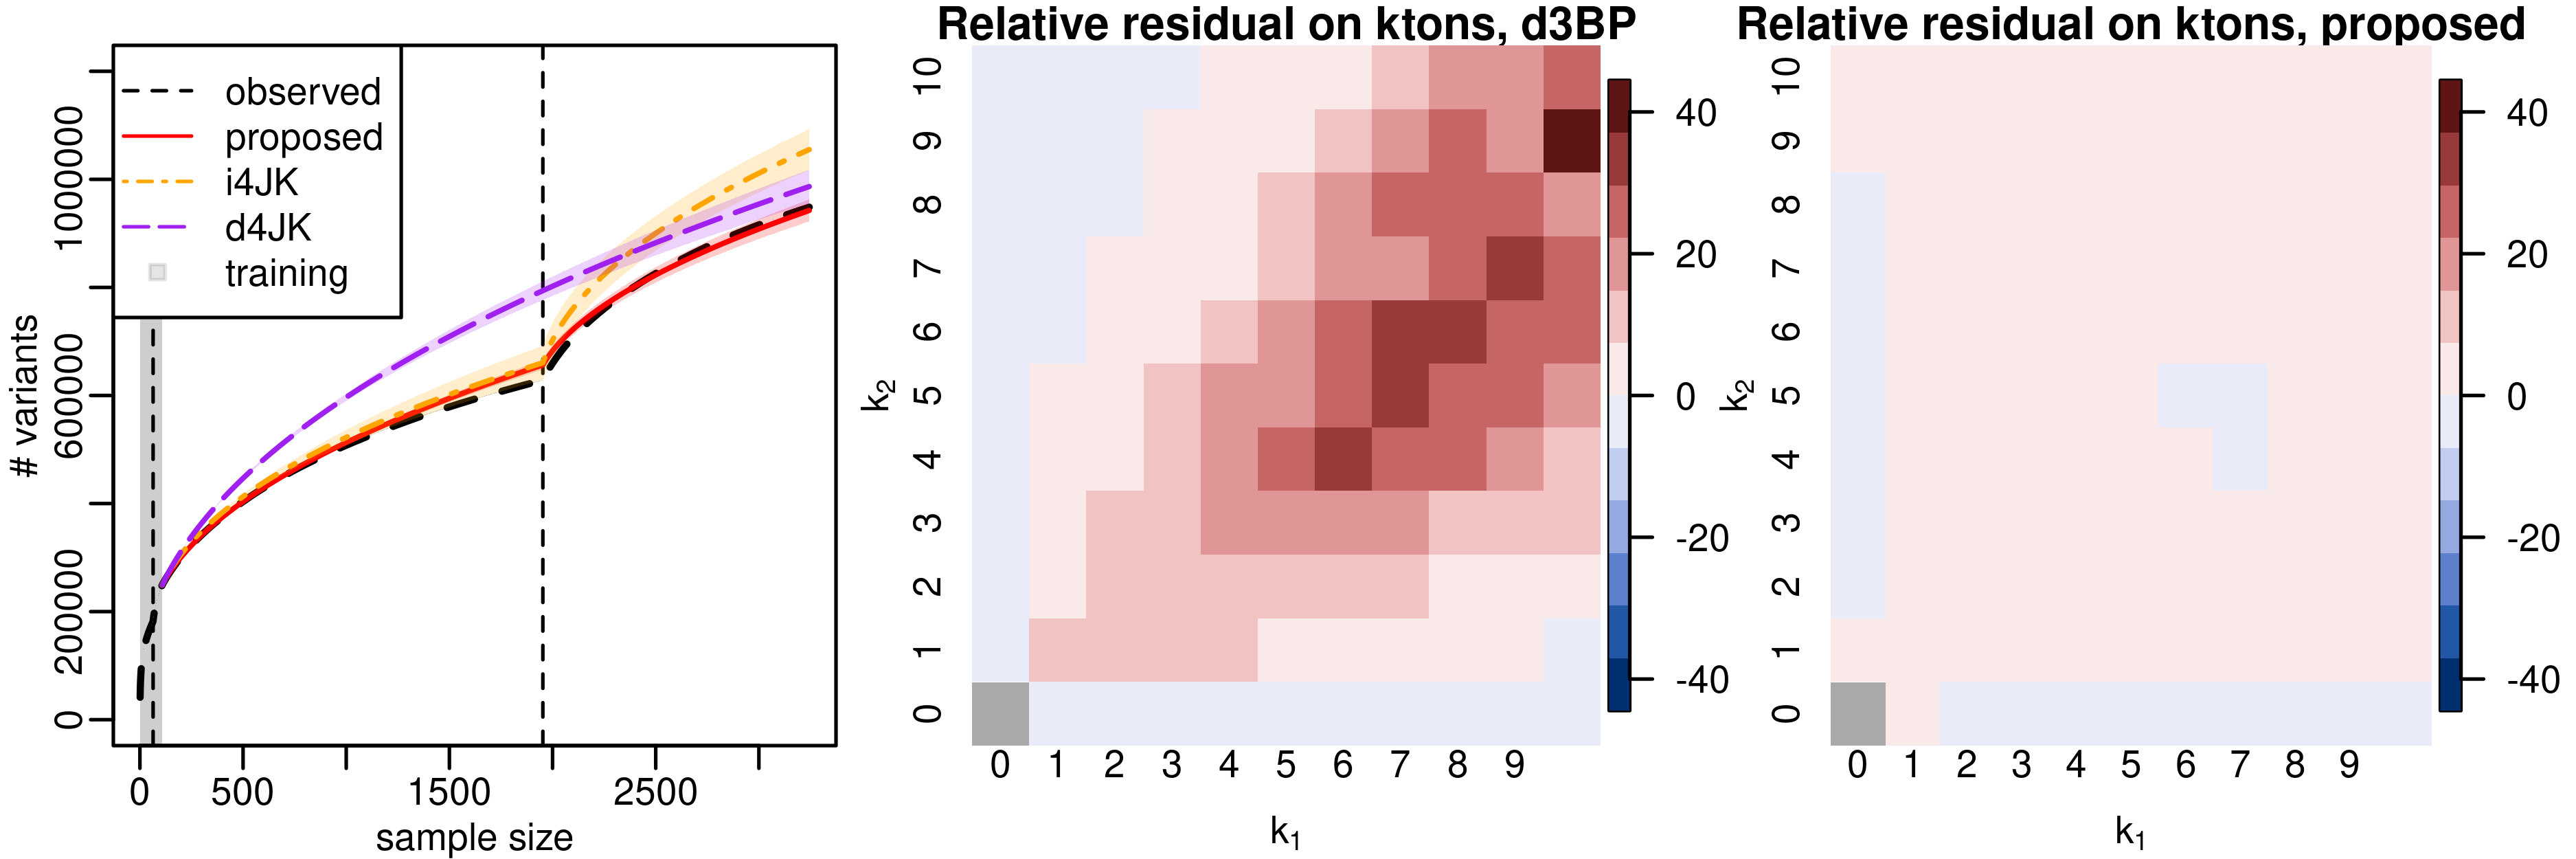
\includegraphics[width = 0.9\textwidth]{Figs/kor_bgr_30fold.png}
    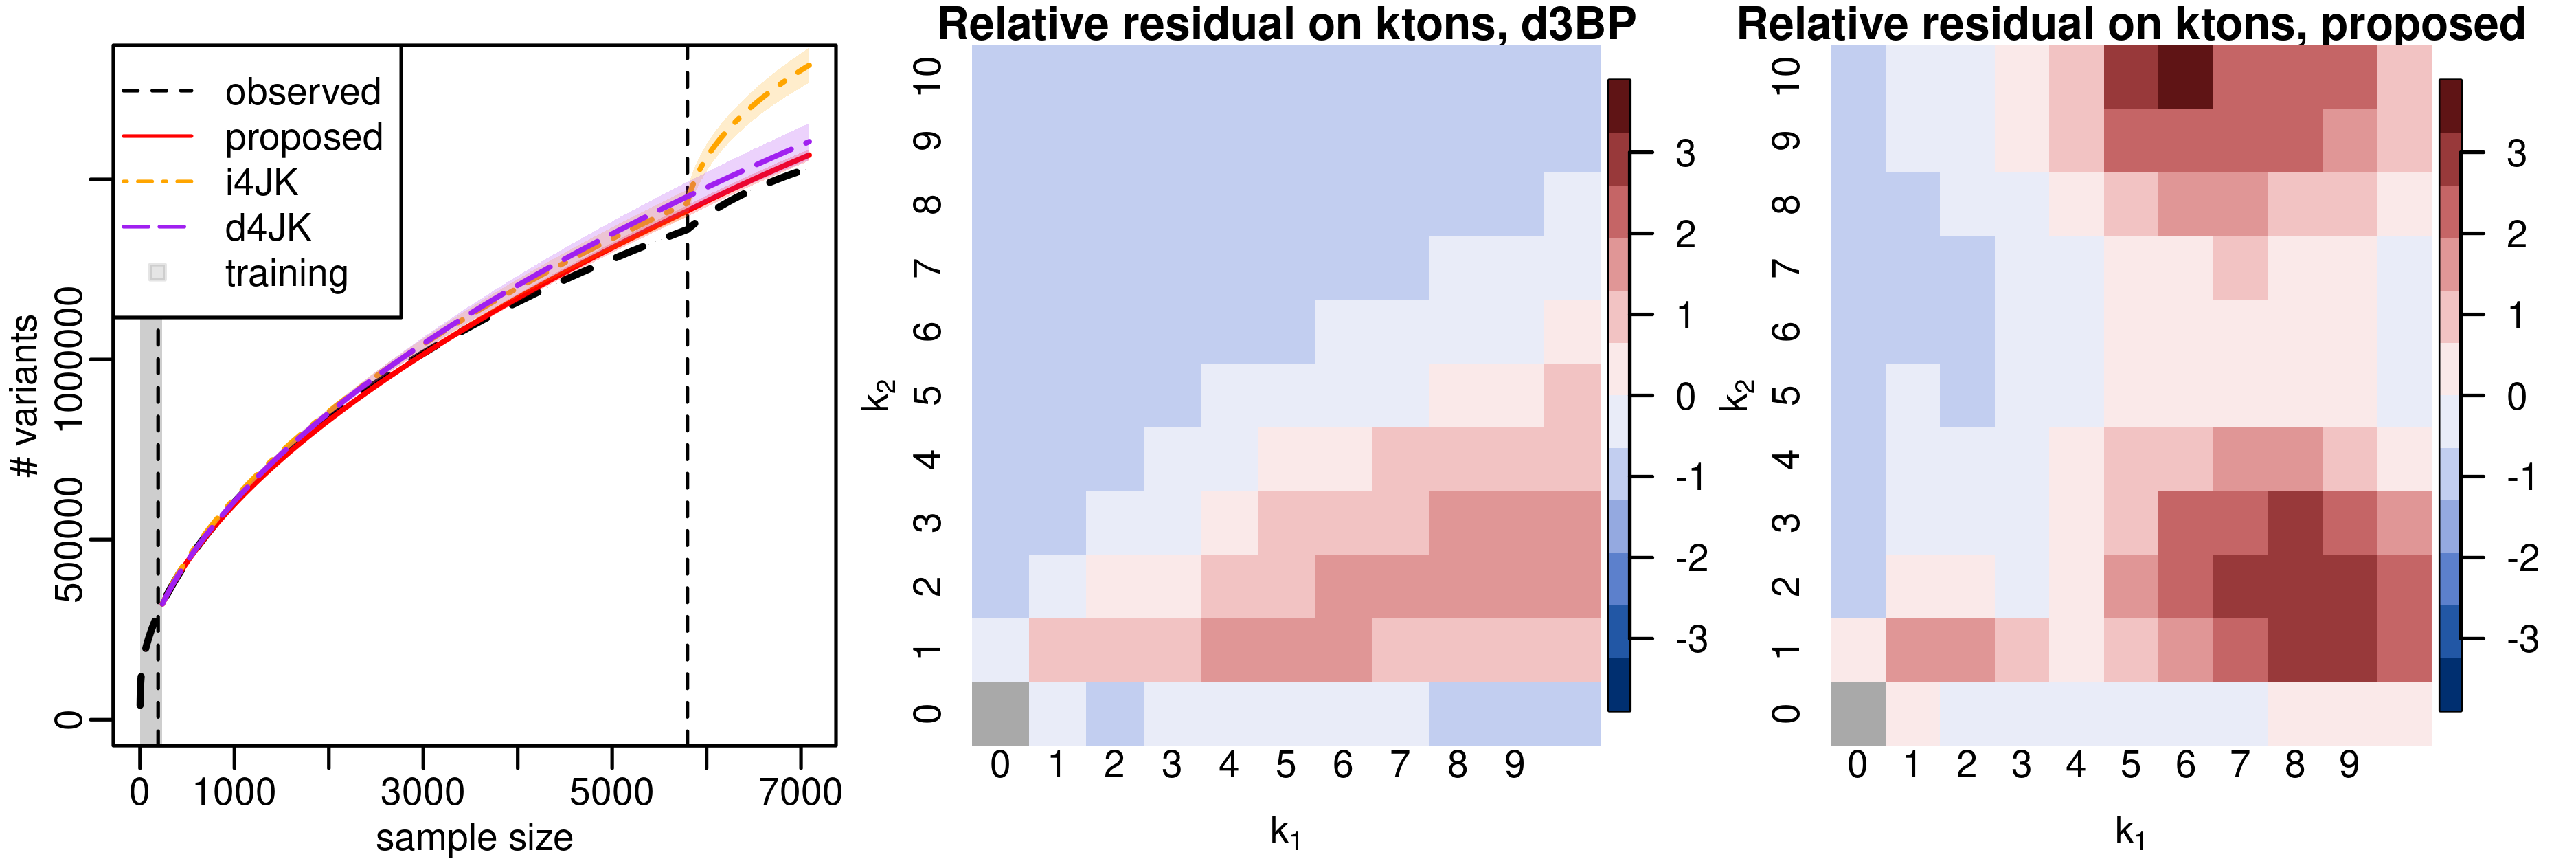
\includegraphics[width = 0.9\textwidth]{Figs/seu_bgr_30fold.png}
    \caption{Predictions for the gnomAD data. The rows correspond to datasets (upper: Korean--Bulgarian, lower: Southern European--Bulgarian). In particular, in the top row, population 1 is Korean, and population 2 is Bulgarian. In the bottom row, population 1 is Southern European, and population 2 is Bulgarian. Other details of the plots are as in \cref{fig:proposed}. We highlight the very different color scales between the upper and lower rows.
    }
   \label{fig:pop_gen}
\end{figure}

